\documentclass[tikz,border=8pt]{standalone}
\usetikzlibrary{positioning,arrows.meta}
\begin{document}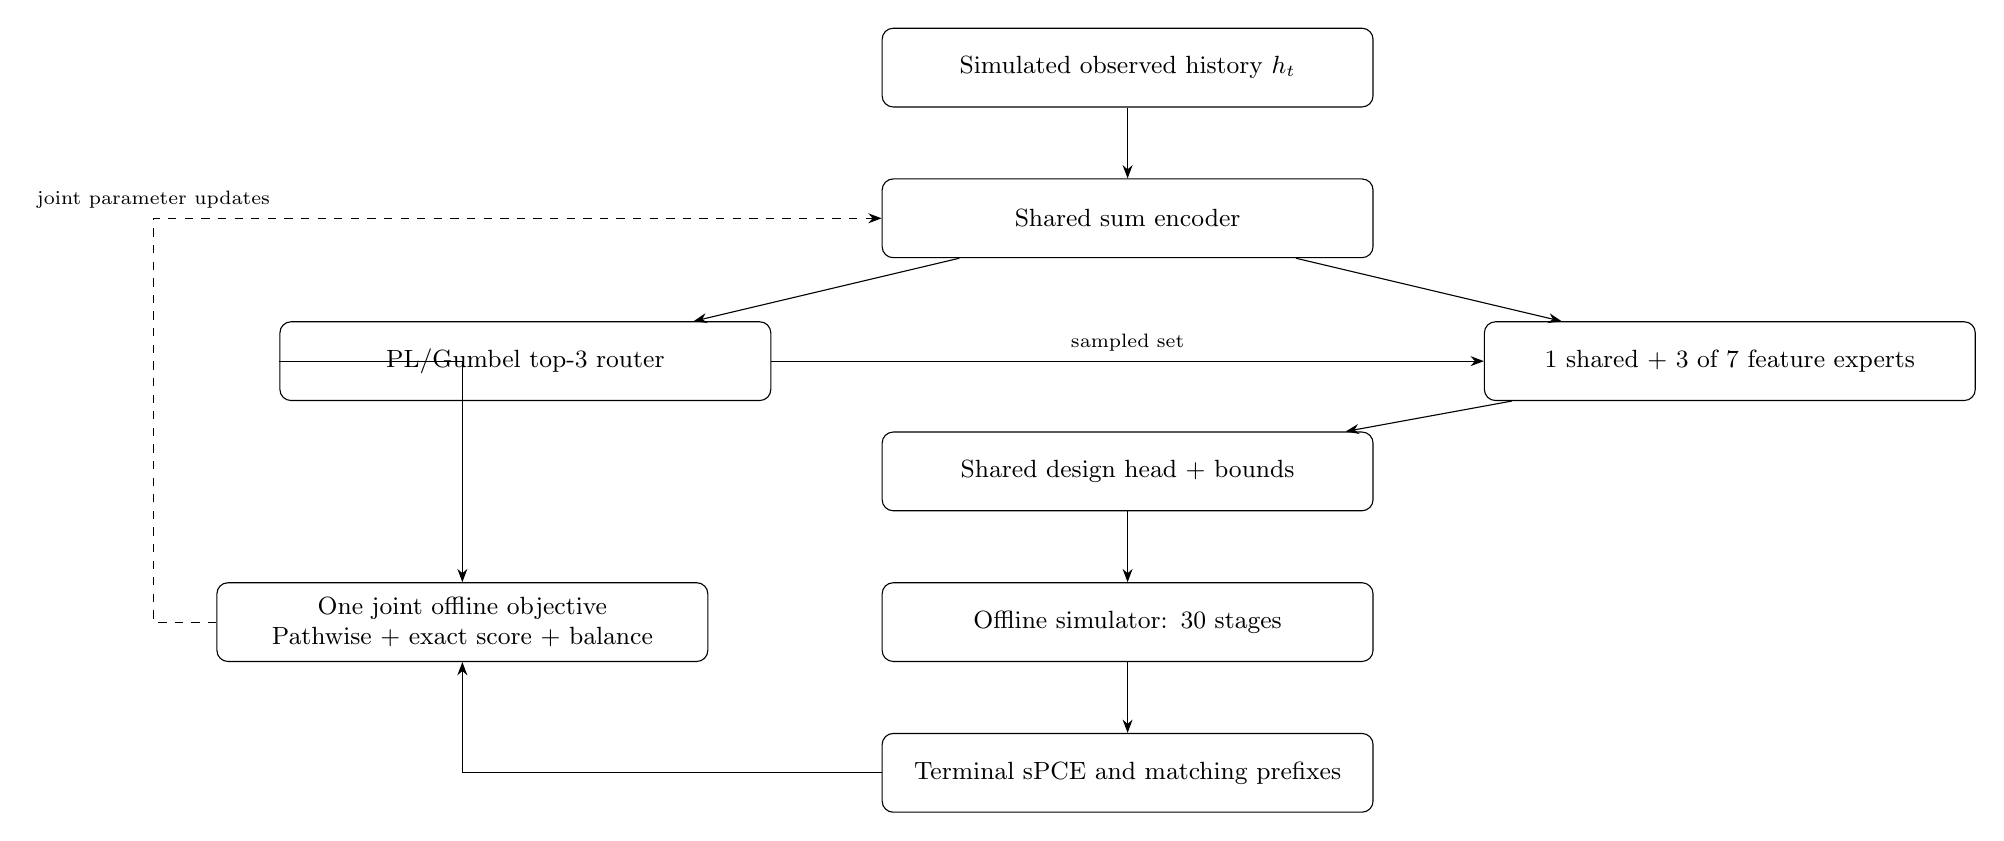
\begin{tikzpicture}[>=Stealth,node distance=9mm,box/.style={draw,rounded corners,align=center,text width=60mm,minimum height=10mm,font=\small}]
\node[box] (h) {Simulated observed history $h_t$};
\node[box,below=of h] (enc) {Shared sum encoder};
\node[box,below left=8mm and 14mm of enc] (router) {PL/Gumbel top-3 router};
\node[box,below right=8mm and 14mm of enc] (experts) {1 shared + 3 of 7 feature experts};
\node[box,below=22mm of enc] (head) {Shared design head + bounds};
\node[box,below=of head] (sim) {Offline simulator: 30 stages};
\node[box,below=of sim] (info) {Terminal sPCE and matching prefixes};
\node[box,left=22mm of sim] (loss) {One joint offline objective\\Pathwise + exact score + balance};
\draw[->] (h)--(enc);\draw[->](enc)--(router);\draw[->](enc)--(experts);
\draw[->](router)--node[above,font=\scriptsize]{sampled set}(experts);
\draw[->](experts)--(head);\draw[->](head)--(sim);\draw[->](sim)--(info);
\draw[->](info)-|(loss);\draw[->](router)-|(loss);
\draw[->,dashed](loss.west)--++(-8mm,0)|-node[above,font=\scriptsize]{joint parameter updates}(enc.west);
\end{tikzpicture}\end{document}
